\documentclass[border=10pt]{standalone}
\usepackage{tikz}
\usetikzlibrary{arrows.meta}

\definecolor{inFill}{RGB}{183,224,177}
\definecolor{inLine}{RGB}{32,102,32}
\definecolor{hidFill}{RGB}{199,203,243}
\definecolor{hidLine}{RGB}{52,58,143}
\definecolor{outFill}{RGB}{243,199,199}
\definecolor{outLine}{RGB}{143,52,52}
\definecolor{lineC}{RGB}{38,44,110}

\begin{document}
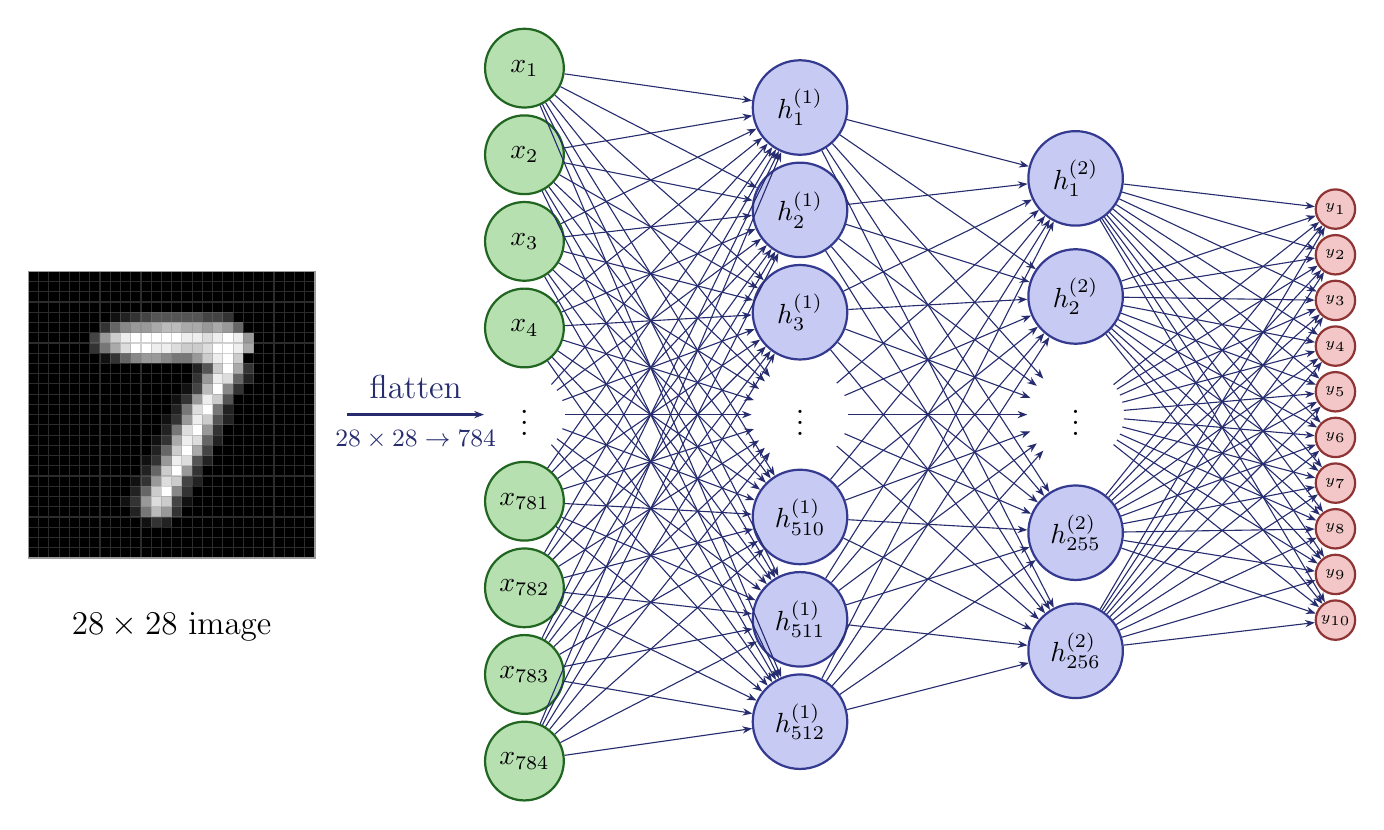
\begin{tikzpicture}[
    >={Stealth[length=3.5pt]}, line width=0.8pt, font=\large,
    inp/.style  ={circle, draw=inLine,  fill=inFill,  minimum size=1.0cm, inner sep=0pt, font=\normalsize},
    hid/.style  ={circle, draw=hidLine, fill=hidFill, minimum size=1.2cm, inner sep=0pt, font=\normalsize},
    outp/.style ={circle, draw=outLine, fill=outFill, minimum size=0.5cm, inner sep=0pt, font=\tiny},
    dots/.style ={circle, minimum size=#1, inner sep=0pt},
    arr/.style  ={lineC, ->, line width=0.4pt},
  ]

  % ---------- 最左：28x28 的数字 7 ----------
  \fill[black] (0,-1.82) rectangle (3.64,1.82);
  \foreach \v [count=\n] in {%
    0,0,0,0,0,0,0,0,0,0,0,0,0,0,0,0,0,0,0,0,0,0,0,0,0,0,0,0,% 行1
    0,0,0,0,0,0,0,0,0,0,0,0,0,0,0,0,0,0,0,0,0,0,0,0,0,0,0,0,% 行2
    0,0,0,0,0,0,0,0,0,0,0,0,0,0,0,0,0,0,0,0,0,0,0,0,0,0,0,0,% 行3
    0,0,0,0,0,0,0,0,0,0,0,0,0,0,0,0,0,0,0,0,0,0,0,0,0,0,0,0,% 行4
    0,0,0,0,0,0,0,0,1,2,3,4,5,5,5,5,5,4,4,3,0,0,0,0,0,0,0,0,% 行5
    0,0,0,0,0,0,0,3,6,8,9,9,10,11,11,10,10,9,10,9,6,0,0,0,0,0,0,0,% 行6
    0,0,0,0,0,0,4,9,12,14,15,15,15,15,15,14,14,13,14,15,14,9,0,0,0,0,0,0,% 行7
    0,0,0,0,0,0,3,7,10,13,15,15,14,14,13,12,12,13,15,15,14,10,0,0,0,0,0,0,% 行8
    0,0,0,0,0,0,0,1,3,6,8,9,9,8,7,7,9,12,14,15,12,0,0,0,0,0,0,0,% 行9
    0,0,0,0,0,0,0,0,0,0,0,0,0,0,0,0,2,5,12,15,10,3,0,0,0,0,0,0,% 行10
    0,0,0,0,0,0,0,0,0,0,0,0,0,0,0,0,3,9,14,13,6,2,0,0,0,0,0,0,% 行11
    0,0,0,0,0,0,0,0,0,0,0,0,0,0,0,1,4,11,15,8,3,0,0,0,0,0,0,0,% 行12
    0,0,0,0,0,0,0,0,0,0,0,0,0,0,1,3,9,14,12,5,0,0,0,0,0,0,0,0,% 行13
    0,0,0,0,0,0,0,0,0,0,0,0,0,0,2,7,13,15,7,2,0,0,0,0,0,0,0,0,% 行14
    0,0,0,0,0,0,0,0,0,0,0,0,0,1,3,9,14,12,5,2,0,0,0,0,0,0,0,0,% 行15
    0,0,0,0,0,0,0,0,0,0,0,0,0,2,7,13,15,9,3,0,0,0,0,0,0,0,0,0,% 行16
    0,0,0,0,0,0,0,0,0,0,0,0,1,3,10,14,13,6,2,0,0,0,0,0,0,0,0,0,% 行17
    0,0,0,0,0,0,0,0,0,0,0,0,2,6,12,15,10,4,0,0,0,0,0,0,0,0,0,0,% 行18
    0,0,0,0,0,0,0,0,0,0,0,1,3,9,14,13,5,2,0,0,0,0,0,0,0,0,0,0,% 行19
    0,0,0,0,0,0,0,0,0,0,0,2,6,12,15,9,3,0,0,0,0,0,0,0,0,0,0,0,% 行20
    0,0,0,0,0,0,0,0,0,0,1,3,9,13,12,4,2,0,0,0,0,0,0,0,0,0,0,0,% 行21
    0,0,0,0,0,0,0,0,0,0,2,6,12,15,8,3,0,0,0,0,0,0,0,0,0,0,0,0,% 行22
    0,0,0,0,0,0,0,0,0,1,3,9,13,12,4,1,0,0,0,0,0,0,0,0,0,0,0,0,% 行23
    0,0,0,0,0,0,0,0,0,0,2,7,11,9,3,0,0,0,0,0,0,0,0,0,0,0,0,0,% 行24
    0,0,0,0,0,0,0,0,0,0,0,1,3,2,0,0,0,0,0,0,0,0,0,0,0,0,0,0,% 行25
    0,0,0,0,0,0,0,0,0,0,0,0,0,0,0,0,0,0,0,0,0,0,0,0,0,0,0,0,% 行26
    0,0,0,0,0,0,0,0,0,0,0,0,0,0,0,0,0,0,0,0,0,0,0,0,0,0,0,0,% 行27
    0,0,0,0,0,0,0,0,0,0,0,0,0,0,0,0,0,0,0,0,0,0,0,0,0,0,0,0 % 行28
  }{%
    \ifnum\v>0\relax
      \pgfmathtruncatemacro{\col}{int(mod(\n-1,28))}
      \pgfmathtruncatemacro{\ybot}{27-int((\n-1)/28)}
      \pgfmathsetmacro{\gpct}{\v/15}
      \definecolor{px}{gray}{\gpct}
      \fill[px] ({0.13*\col}, {-1.82+0.13*\ybot}) rectangle ++(0.13,0.13);
    \fi
  }
  \draw[gray, opacity=0.35, thin, step=0.13] (0,-1.82) grid (3.64,1.82);
  \draw[gray!80, line width=0.5pt] (0,-1.82) rectangle (3.64,1.82);
  \node at (1.82,-2.7) {$28\times 28$ image};

  % ---------- 输入层 784：小圆(1.0cm)画 9 个，列最高 ----------
  \node[inp]  (in1)   at (6.3, 4.4) {$x_1$};
  \node[inp]  (in2)   at (6.3, 3.3) {$x_2$};
  \node[inp]  (in3)   at (6.3, 2.2) {$x_3$};
  \node[inp]  (in4)   at (6.3, 1.1) {$x_4$};
  \node[dots=1.0cm] (inV) at (6.3, 0) {$\vdots$};
  \node[inp]  (in781) at (6.3,-1.1) {$x_{781}$};
  \node[inp]  (in782) at (6.3,-2.2) {$x_{782}$};
  \node[inp]  (in783) at (6.3,-3.3) {$x_{783}$};
  \node[inp]  (in784) at (6.3,-4.4) {$x_{784}$};

  % ---------- 隐藏层 512：画 7 个 ----------
  \node[hid]  (h11)   at (9.8, 3.9) {$h_1^{(1)}$};
  \node[hid]  (h12)   at (9.8, 2.6) {$h_2^{(1)}$};
  \node[hid]  (h13)   at (9.8, 1.3) {$h_3^{(1)}$};
  \node[dots=1.2cm] (h1V) at (9.8, 0) {$\vdots$};
  \node[hid]  (h1510) at (9.8,-1.3) {$h_{510}^{(1)}$};
  \node[hid]  (h1511) at (9.8,-2.6) {$h_{511}^{(1)}$};
  \node[hid]  (h1512) at (9.8,-3.9) {$h_{512}^{(1)}$};

  % ---------- 隐藏层 256：画 5 个 ----------
  \node[hid]  (h21)   at (13.3, 3.0) {$h_1^{(2)}$};
  \node[hid]  (h22)   at (13.3, 1.5) {$h_2^{(2)}$};
  \node[dots=1.2cm] (h2V) at (13.3, 0) {$\vdots$};
  \node[hid]  (h2255) at (13.3,-1.5) {$h_{255}^{(2)}$};
  \node[hid]  (h2256) at (13.3,-3.0) {$h_{256}^{(2)}$};

  % ---------- 输出层 10：全画，列最矮 ----------
  \foreach \i in {1,...,10}
    \node[outp] (o\i) at (16.6, {2.61-0.58*(\i-1)}) {$y_{\i}$};

  % ---------- 展平箭头 ----------
  \draw[lineC, ->, line width=1pt] (4.05,0) -- (inV)
    node[midway, above=2pt] {flatten}
    node[midway, below=2pt, font=\small] {$28\times28 \to 784$};

  % ---------- 全连接 ----------
  \foreach \i in {in1,in2,in3,in4,inV,in781,in782,in783,in784}
    \foreach \j in {h11,h12,h13,h1V,h1510,h1511,h1512}
      \draw[arr] (\i) -- (\j);
  \foreach \i in {h11,h12,h13,h1V,h1510,h1511,h1512}
    \foreach \j in {h21,h22,h2V,h2255,h2256}
      \draw[arr] (\i) -- (\j);
  \foreach \i in {h21,h22,h2V,h2255,h2256}
    \foreach \j in {1,...,10}
      \draw[arr] (\i) -- (o\j);

  % % ---------- 层名放底部 ----------
  % \node[align=center] at (6.3,-6.1)  {input\\ $784$};
  % \node[align=center] at (9.8,-6.1)  {hidden 1\\ $512$};
  % \node[align=center] at (13.3,-6.1) {hidden 2\\ $256$};
  % \node[align=center] at (16.6,-6.1) {output\\ $10$};
\end{tikzpicture}
\end{document}